
	\subsection{Electron Transport Measurement using Complex Impedance}
	A four-point impedance measurement measures complex impedance of the IDE sample under test (device under test, or DUT).  
	Impedance measurements follow a temperature dependence derived from models of electron transport under an AC potential.  
	Complex impedance and temperature measurements are used to solve electron mobility under the AC electron transport model detailed below.  
	Temperature measurements were limited to those measurements taken during cool-down of the DUT, since temperature measurements during fast heating of the sample carry very large errors.  
	Measurements of impedance over temperature during cool-down (FIGURE "cooldown\_residuals") were identical within uncertainties for the Au$_25$ sample (JD04) and a bare IDE sample (JD05), and electron mobility will be identical.  
	Electron mobility calculated for the Au$_25$ (JD04) sample was ${\epsilon\over{k}} = 1.1e+04 K$, $\epsilon = 0.96 eV$.
		
	\subsubsection{Introduction: Measurement of Complex Impedance} 
	DC resistance measurements of the electrode show only its insulating properties, as the glass substrate is a poor conductor and the IDE is a weak capacitor, so AC resistance is measured.
	AC resistance in the IDE samples follows the temperature-dependent electron mobility.
	
	\begin{equation}
		R = R_0 \cdot e^{\epsilon\over{k \cdot T}}
		\label{eq:emobility}
	\end{equation}
	
	This equation can be rearranged into a linear equation to solve for $\epsilon$.
	
	\begin{equation}
		ln(R) = {\epsilon\over{k}} {1\over{T}} - ln(R_0)
		\label{eq:solve_emobility}
	\end{equation}
	
	${\epsilon\over{k}}$ and $ln(R_0$ are found by least-squared fit of the linear portion of the data.
	
	\begin{figure}
	
	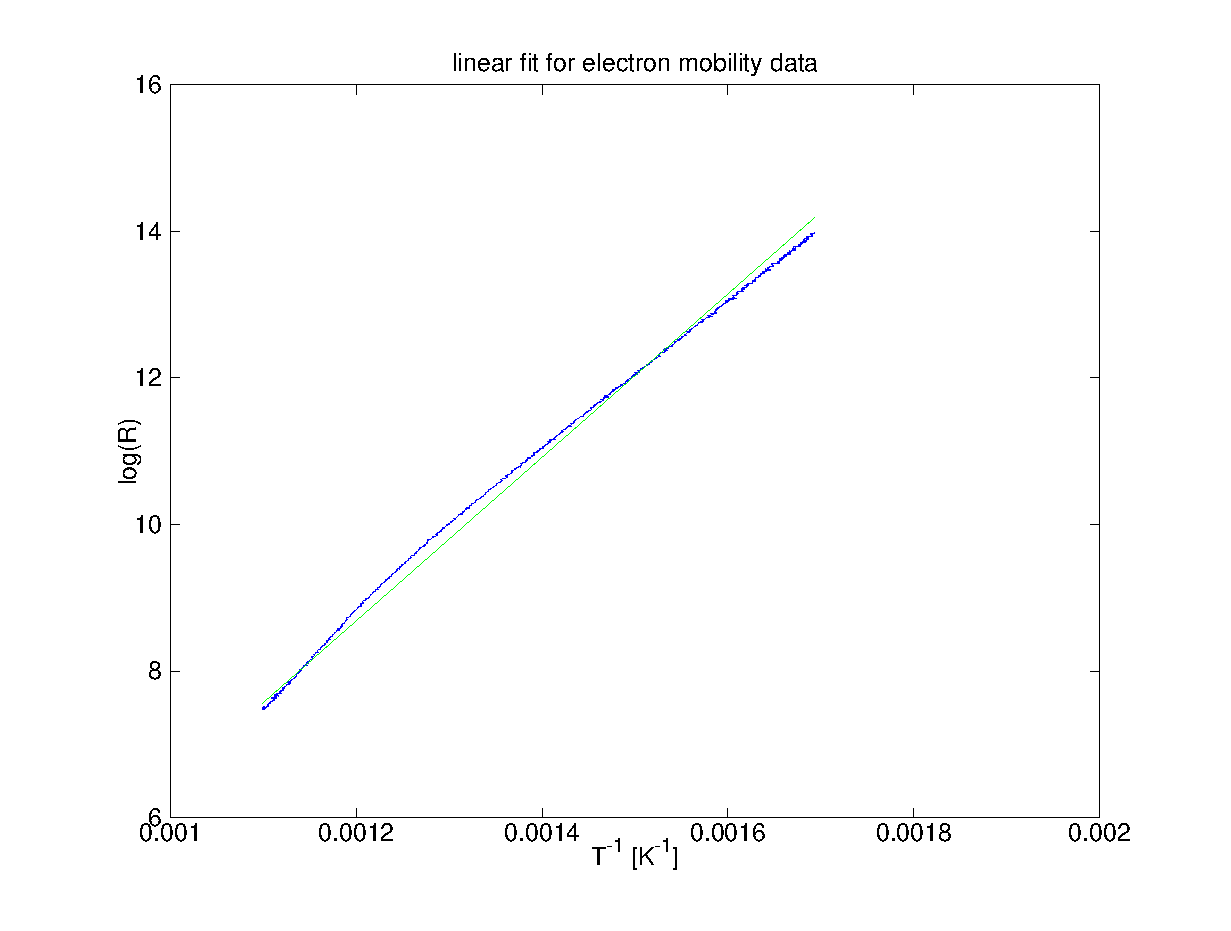
\includegraphics[scale=0.4]{images/electron_mobility.eps} 
	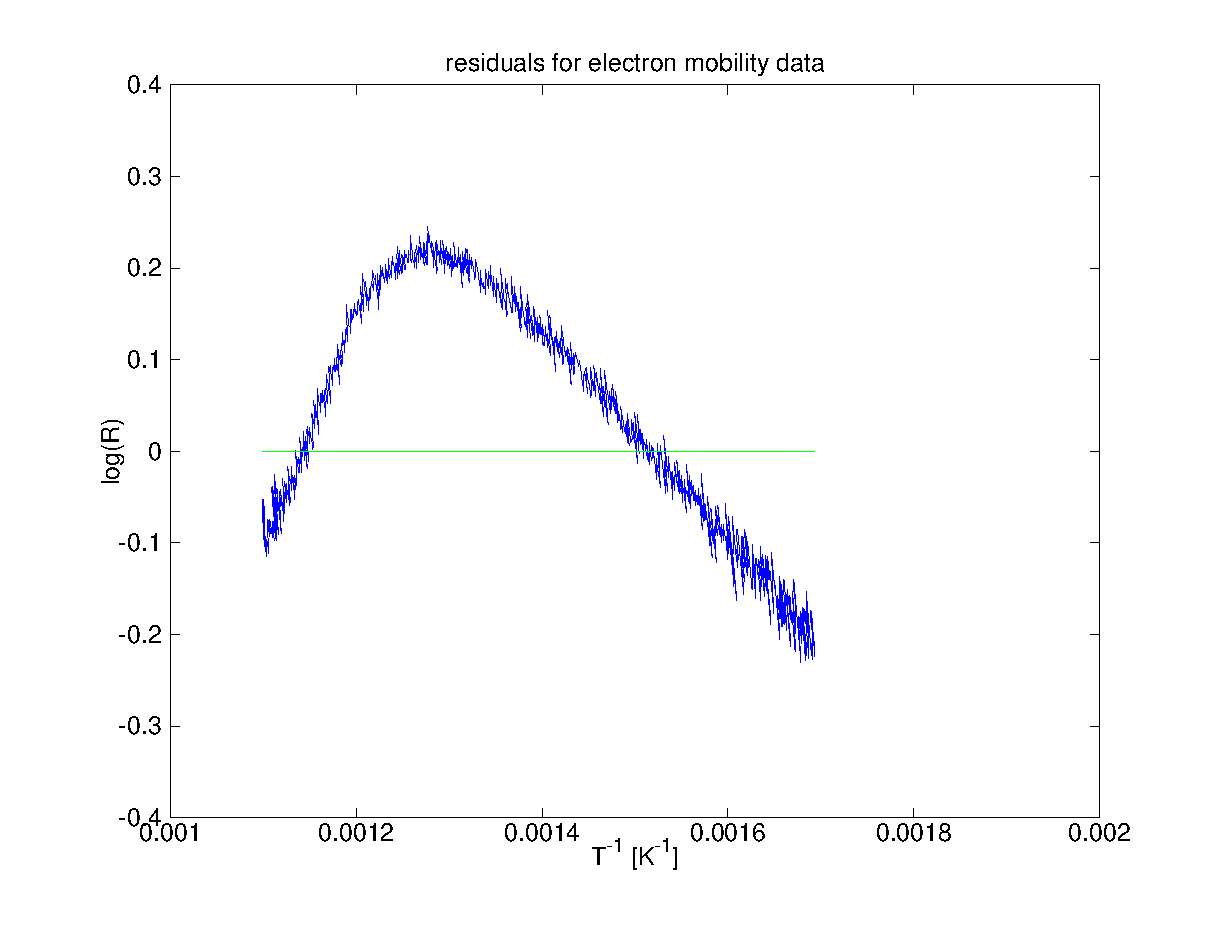
\includegraphics[scale=0.4]{images/electron_mobility_residual.eps}
	\label{f:emobility}
	\caption{During cool-down of the sample, the impedance versus temperature measurements are well-sampled, and can be used to solve for electron mobility.  ${\epsilon\over{k}} = 1.1e+04 K$, $\epsilon = 0.96 eV$, $R_0 = 9.1e-3\Omega$.  Error bars are needed, and will have magnitude at least proportional to the fit residuals.}
	\end{figure}
	The temperature range observed is between $295K$ and $900K$, 
	
	Sample resistance (a parallel AC resistance) is typically high for the sample under test, this resistance changes when the sample is heated and the polymers are burned off.  

	The resistance $R_p$ of a high-resistance sample can be measured from the complex impedance $(Z,\theta)$ by Equation ~\ref{eq:R_p}.  Use of the parallel resistance $R_p$ is justified at high sample resistance because the series resistance $R_s$ of the test leads and contacts are orders of magnitude smaller.
	
	\begin{equation}
		R_p = {{Z} \over {cos({\theta})}}
		\label{eq:R_p}
	\end{equation}
	
	Typical values for complex impedance measured by the auto-balancing bridge method via an Agilent 82XX LCR meter are as follows.
	
	\begin{equation}
		\left( Z,\theta,\nu,T \right) = \left( 15 M\Omega, -89.9^\circ, 1kHz, 22^{\circ}C \right)
	\end{equation}
	\begin{equation}
		\left( Z, \theta, \nu, T \right) = \left( 800 k\Omega, -88^\circ, 45kHz, 22^{\circ}C \right)
	\end{equation}
	
	This result shows that the $R_p$ ``resistance'' component (which is $Z$ divided by $cos(-89^\circ)$) is immeasurably high at low frequencies and low temperature.  It is only at higher temperatures that $R_p$ drops to the measurable range, and this occurs at about $250^{\circ}C$ when the impedance phase angle $\theta$ drops from $-89.9^\circ$ towards $0.1^\circ$.
	
	During the burn-off of the polymers, the parallel resistance may drop to under 100 ohms, which requires a four-point measurement to compensate for the series resistance test lead impedance.
	A four-point measurement is necessary because the test leads have been reported (AD5933) to have up to kilo-ohm impedance when measuring low sample resistance.


